%        File: nandflash.tex
%     Created: ���� ���� 04 02:00 ���� 2012 CST
% Last Change: ���� ���� 04 02:00 ���� 2012 CST
%
\documentclass[a4paper]{article}
\usepackage{graphicx}
\usepackage{indentfirst}
\usepackage{algorithm}
\usepackage{xcolor}
\usepackage{listings}

\definecolor{dkgreen}{rgb}{0,0.6,0}
\definecolor{gray}{rgb}{0.5,0.5,0.5}
\definecolor{mauve}{rgb}{0.58,0,0.82}

\lstset{ %
  basicstyle=\footnotesize,           % the size of the fonts that are used for the code
  numbers=none,                   % where to put the line-numbers
  numberstyle=\footnotesize,          % the size of the fonts that are used for the line-numbers
  stepnumber=2,                   % the step between two line-numbers. If it's 1, each line
                                  % will be numbered
  numbersep=5pt,                  % how far the line-numbers are from the code
  backgroundcolor=\color{white},      % choose the background color. You must add \usepackage{color}
  showspaces=false,               % show spaces adding particular underscores
  showstringspaces=false,         % underline spaces within strings
  showtabs=false,                 % show tabs within strings adding particular underscores
  frame=none,                   % adds a frame around the code
  tabsize=2,                      % sets default tabsize to 2 spaces
  captionpos=b,                   % sets the caption-position to bottom
  breaklines=true,                % sets automatic line breaking
  breakatwhitespace=false,        % sets if automatic breaks should only happen at whitespace
  title=\lstname,                   % show the filename of files included with \lstinputlisting;
                                  % also try caption instead of title
  numberstyle=\tiny\color{gray},        % line number style
  keywordstyle=\color{blue},          % keyword style
  commentstyle=\color{dkgreen},       % comment style
  stringstyle=\color{mauve},         % string literal style
  escapeinside={\%*}{*)},            % if you want to add a comment within your code
  morekeywords={*,...}               % if you want to add more keywords to the set
}


\begin{document}
\title{The Implementation of Nandflash Software Stack}
\author{Chen Yuheng \\ Tsinghua Unv.}

\maketitle

\section{Structure of Nandflash}
Flash memory is a non-volatile computer storage chip that can be electrically erased and reprogrammed.\cite{WIKI_NAND}
The high density NAND type must also be programmed and read in (smaller) blocks, or pages.
Most NAND chip nowadays supports 2kB pages, which is called large page NAND. NAND flash can
only be programmed page by page, and erased block by block (generally speaking, a block contains
32 or 64 pages). 

One of the most important characteristic of NAND is its unreliability, which is shown in the 
following three aspects:
\begin{enumerate}
  \item Bit inversion;
  \item Bad blocks before the chip is shipped (intristic bad blocks);
  \item Bad blocks caused by erasing or programming.
\end{enumerate}

This characteristic leads to the special physical structure of NAND flash chip,
which is shown in Fig. \ref{fig:nand}\cite{NAND_DATASHEET}. The spare area on
a NAND chip enables users to store ECC and other metadata to overcome the 
unreliability of NAND.

\begin{figure}[h]
  \centering
  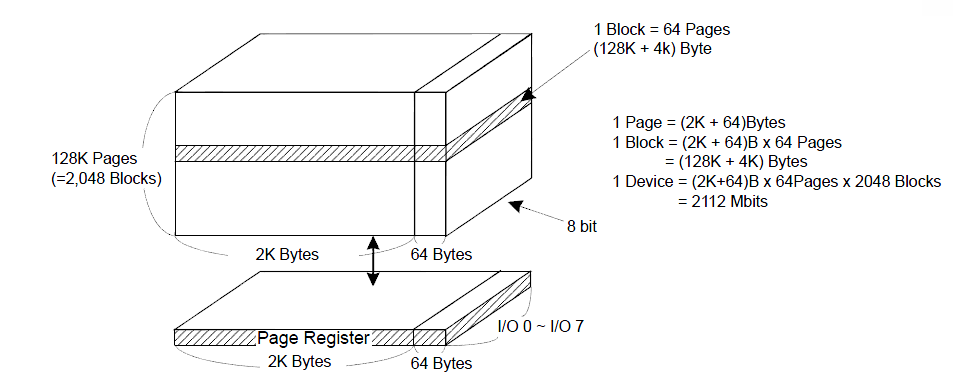
\includegraphics[width=0.9\linewidth]{nand.png}
  \caption{NAND Flash Structure}
  \label{fig:nand}
\end{figure}

Our implementation is tested on a K9F2G08U0M chip with an ARM9 controller.
Information about this chip can be found in its datasheet:

\begin{verbatim}
- Memory Cell Array
-X8 device(K9F2G08X0M) : (256M + 8,192K)bit x 8bit
- Data Register
-X8 device(K9F2G08X0M): (2K + 64)bit x8bit
- Cache Register
-X8 device(K9F2G08X0M) : (2K + 64)bit x8bit
\end{verbatim}

In order to design a general NAND flash driver, a abstract view of 
NAND flash memory model is essential. A NAND flash driver uses 
the following operations to control the NAND chip:
\begin{itemize}
  \item  Erase a block ( change bits from 0 to 1)
  \item  Program a page ( change bits from 1 to 0)
  \item  Read a page (page size = main area + spare area)
  \item  ECC calculation
  \item  ECC correction 
\end{itemize}

Our source code is available on GitHub
\footnote{https://github.com/chyh1990/ucore-arch-arm}.

\section{Overview of Nandflash Software Stack}
Our NAND software stack design is similar to Linux's, but simplified for
embedded system. Our implementation is built based on an experimental
operating system, which provides infrastructure of memory management and
Virtual File System(VFS).

The structure of our  Nandflash Software Stack is illustrated in Fig.\ref{fig:soft}.
\begin{figure}[h]
  \centering
  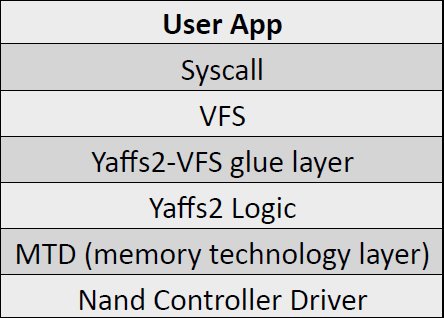
\includegraphics[width=0.6\linewidth]{soft.png}
  \caption{Nand Software Stack in Ucore}
  \label{fig:soft}
\end{figure}


\section{Implementation Details}
\subsection{Nand Controller Driver}
Controller driver is the lowest layer of the software stack -- it communicates 
with the hardware directly. Thus, this part is chip specific. This layer
should implement several interfaces provided in the structure \emph{nand\_chip}:

\begin{algorithm}[H]
   \begin{lstlisting}[language={C++}]
struct nand_chip {
  void (*write_cmd)(unsigned char cmd);
  void (*write_addr)(unsigned char addr);
  void (*enable_chip)(int enable);
  unsigned char (*read_byte)();
  void (*write_byte)(unsigned char byte);
  void (*wait_rdy)();
  void (*write_full_addr)(unsigned int row, unsigned int col);

  int (*ecc_calculate)(const unsigned char *dat, size_t sz, unsigned char *ecc_code);
  int (*ecc_correct)(unsigned char *dat,unsigned char *read_ecc, unsigned char *isnull);
/* ... */
};
\end{lstlisting}
  \caption{kern-ucore/fs/nand\_mtd.h}
\end{algorithm}


\subsection{Memory Technology Device(MTD) Layer}
MTD layer take responsibility for the following tasks:
\begin{itemize}
  \item 
Manages partitions on a nandflash chip
  \item
Organizes OOB area (spare area) layout
  \item
Provides interfaces to read/write a page and erase a block 
  \item
Mark/Check a bad block
\end{itemize}

Again, the structure \emph{nand\_chip} take care of MTD layer operations, as shown
in Alg. \ref{alg:nc}.

\begin{algorithm}[h]
   \begin{lstlisting}[language={C++}]
struct nand_chip {
/* ... */
  /* size of data buffer>=pg_size, size of spare buffer>=spare_size */
  int (*read_page)(struct nand_chip* chip,unsigned page_id, 
    unsigned char *data,unsigned char *spare, int *eccStatus);

  /* spare data only contain user data, ecc auto-appended */
  int (*write_page)(struct nand_chip* chip, unsigned pageId, 
					  const unsigned char *data, unsigned dataLength,
            const unsigned char *spare, unsigned spareLength);

  int (*erase_block)(struct nand_chip* chip, unsigned blkID);
  /* return 0 if bad */
  int (*check_block)(struct nand_chip *chip, unsigned blkID);
  /* mark bad blk */
  int (*mark_badblock)(struct nand_chip *chip, unsigned blkID);

  struct nand_ecclayout *ecclayout; 

  int badblock_offset;
  unsigned spare_size;
  unsigned blk_cnt;
  unsigned pages_per_blk;
  unsigned blk_shift;
  unsigned pg_size;
  unsigned pg_size_shift;
};
\end{lstlisting}
  \caption{kern-ucore/fs/nand\_mtd.h}
  \label{alg:nc}
\end{algorithm}

This structure is so important that it is the center of NAND software stack design.
An implementation example can be found in \emph{kern-ucore/arch/arm/mach-at91/at91-nandflash.c}.

\subsection{Filesystem -- YAFFS2}
Due to NAND's special physical structure, a number of NAND-specific filesystems are designed.
YAFFS2\footnote{http://www.yaffs.net/} is a popular one used in a wide range of embedded system, including Android.

YAFFS stands for Yet Another Flash File System. YAFFS is the first file system that has been  designed, from the ground up, for NAND storage.
In 2002 Aleph One set out to identify file system options for using NAND Flash as a file system. Various file systems available at the time were evaluated and all were found lacking in one way or another. The need for a suitable NAND storage file system was identified and YAFFS was designed to fill that need.\cite{YAFFS2}

YAFFS2 supports several important features:
\begin{itemize}
  \item Linux-compatible VFS interface
  \item POSIX interface
  \item Wear Leveling Algorithm
  \item Bad block handling
\end{itemize}

However, although YAFFS2 provides both Linux VFS and POSIX interface, they are
not usable by \emph{ucore}.
Ucore��s VFS is not compatible with Linux��s, so we have to rewrite all code for this layer\footnote{see fs/yaffs2\_direct/yaffs\_vfs.[hc]}.
But fortunately, the lower layer API of YAFFS2 provides \emph{yaffs\_obj}, functionally equivalent to \emph{inode}.
Thus, generally speaking, functions in this layer map \emph{inode} requests to \emph{yaffs\_obj} manipulation.

\section{Configuration Guide}
In order to use a NAND device on your platform, you need to provide 
your driver and MTD implementation as mentioned in the last section.

Besides, you have to configure your NAND partition in \emph{fs/yaffs2\_direct/mtd\_glue.c}:
\begin{verbatim}
  static struct mtd_partition partition[] = {
    { "boot", 0, 9 },
    { "data", 10, 0x400}, //128M = 0x400*64*2K
  };
\end{verbatim}

You may want to format (erase) the partition you want to use first, just call:
\begin{verbatim}
  void mtd_erase_partition(struct nand_chip*chip ,const char* name);
\end{verbatim}

Where \emph{name} is your partition name.
Then, change:
\begin{verbatim}
static const char *mount_partition = "/data";
\end{verbatim}
to the partition name you want to mount.

After that, you should initialize YAFFS2 in \emph{init.c}:
\begin{verbatim}
  yaffs_start_up();
  yaffs_vfs_init();
\end{verbatim}

On the other hand, if you want to debug YAFFS2 or the VFS glue layer
in \emph{Qemu}, you can use the following initialization code:
\begin{verbatim}
  yaffsfs_OSInitialisation();
  yramsim_CreateRamSim("data", 1,20, 2, 16);
  yaffs_vfs_init();
\end{verbatim}
It will create a YAFFS2 Ramdisk and mount it. Note that this will bypass all 
the MTD layer and driver code, so you will have to find out
other techniques to debug it.

That's all, your NAND will be mounted to \emph{disk1:/} by default,
try this in ucore's shell:

\begin{verbatim}
  cd disk1:/
  ls
\end{verbatim}


\section{Conclusion}
This document is a part of our OS course project. If you feel like 
to use this NAND software stack in your work, I hope this document 
will help you. For the code is only tested on AT91SAM9 CPU and 8-bit NAND
flash, it might refuse to work without modifications.

\bibliographystyle{IEEEtran}
\bibliography{book}

\end{document}


